\documentclass[onecolumn,a4paper,amsmath,amssym,pre]{revtex4}
\usepackage{graphicx}% Include figure files
\usepackage{dcolumn}% Align table columns on decimal point
\usepackage{subfigure}
\usepackage{bm}% bold math
\bibliographystyle{pf}
\usepackage{setspace}
\usepackage{fancyhdr}
\usepackage{amsmath}
\usepackage{color}
\usepackage{epstopdf}
\usepackage{booktabs}
\usepackage{xcolor}
\usepackage{hyperref}
\usepackage{ulem}
\usepackage[abs]{overpic}

\addtolength{\parskip}{0pt}
\addtolength{\floatsep}{0pt}
\addtolength{\textfloatsep}{0pt}
\addtolength{\abovecaptionskip}{0pt}
\addtolength{\belowcaptionskip}{0pt}
%\newcommand{\ra}[1]{\renewcommand{\arraystretch}{#1}
\newcommand{\volume}{{\ooalign{\hfil$V$\hfil\cr\kern0.08em--\hfil\cr}}}




\begin{document}
    

\begin{tabular}{ r | l }
  \hline            
   \textbf{Manuscript Number}:& CAF-D-24-00627 \\	
   \textbf{Title}: & Optimizing fluid mixing in channel flow using wall-mounted flexible structures\\
%	\textbf{Revision title}: & Generating periodic vortex pairs using flexible structures \\  
  \textbf{Authors}:  & Gaurav Singh, Arahata Senapati, Arnab Atta and Rajaram Lakkaraju \\
  \hline  
\end{tabular}\\ \\



%	\textcolor{red}{\textbf{Editor: Raghuraman N. Govardhan}}\\
	
	{\color{red}
Dear Dr. Rajaram Lakkaraju,\\

Attached are the reviews of your paper entitled
"Optimizing fluid mixing in channel flow using wall-mounted flexible structures" which was submitted for publication in Computers and Fluids.

If the article is revised in accordance with these reviews, we shall be glad to reconsider it for publication. Please respond to the specific comments of the referees in a separate document. It would be appreciated if you could submit your revised paper by Jan 14, 2025. If additional time is needed to complete the revision I would be most grateful if you would let me know.

If you are submitting a revised manuscript, please also:

a) outline each change made (point by point) as raised in the reviewer comments

AND/OR

b) provide a suitable rebuttal to each reviewer comment not addressed\\
	
	  \color{black}{\textbf{Reply}: Thank you for providing valuable feedback on my manuscript. I have carefully read the reviewers' reports and appreciate the constructive comments provided. I would like to express my gratitude to the reviewers for their thorough evaluation of the manuscript. I understand the importance of their insights in enhancing the quality of the work. I have tried to address each of the reviewers' comments diligently in a rebuttal document quoting each of the reviewers' comments in full.
	  	
	  In the revised version of the manuscript, I have incorporated the suggested modifications and improvements. Furthermore, as per your recommendation, I have submitted two versions of the revised manuscript. One version includes the changes made, highlighted using a different font color, and the other is a clean revised version for easier assessment.
	  	
	  %Additionally, we would like to inform you that we wish to add Dr. Leixin Ma to the authorship list of the revised manuscript. Dr. Leixin significantly contributed to the review process by providing valuable insights, critical feedback, and additional computational resources that enhanced the quality of our work. We believe her contributions merit inclusion as a co-author, in accordance with authorship guidelines.
	  
	  I would like to express my appreciation for the guidance provided on the submission process. I sincerely value the opportunity to contribute to the Computer and Fluids journal, and I am dedicated to producing a revised manuscript that meets the high standards of the journal.}\\
	  
	  \vspace{1cm} 
	  Yours sincerely, \\
	  \vspace{0.1cm} \\
	  Dr. Rajaram Lakkaraju \\
	  \today \\
	  IIT Kharagpur, India.
	
\newpage

%--------------------------------------------------
\section*{\textbf{The first referee's comments and actions taken in that regard}}

\textcolor{red}{The authors use wall-mounted flexible structures to optimize fluid mixing in channel flow within a laminar regime. The topic is interesting, the goal of the paper is clearly stated, and the paper can be considered for publication after addressing the following mandatory remarks:}

\begin{enumerate}	
	
	\item \textcolor{red}{The authors consider a mixing index (MI) based on the standard deviation of concentration in a cross-sectional plane perpendicular to the flow direction. I strongly suggest computing the degree of mixing ($\Delta$m), as defined, for example, in Antognoli et al. (2022), by considering the flux of the concentration distribution (because the velocity profile is not uniform in the cross section). Please compare the results in the revised version of the paper. Are the results consistent?}
	
\textbf{Reply}: Thank you for additional insight on the mixing measurement method. The suggested works are insightful and indeed worth comparing with our results. We recalculated the mixing index in our work in terms of the "degree of mixing" which accounts for the flux of the bulk-mixing average mass fraction. We found our results to be consistent with this approach in terms of the trends but with a shift in scale. Since, we have considered long time-averaged $phi$ in our formulation, it reduces the possibility of trend variation in mixing measurement and diminishes the impact of mass flux fluctuations. We have added the following results and discussion in our revised manuscript:

"\textit{According to this method, the `Mixing Index' ranges from $0$ to $1$ where $MI=1$ represents a completely mixed solution and $MI=0$ represents the fully unmixed scalar field. In our formulation, we have considered the time averaged $phi$ in the steady state to diminish any statistical fluctuations. For comparison, we have also computed an alternative mixing metric called 'degree of mixing' based on the flux of bulk or cup-mixing average mass fraction as described in \cite{Antognoli, Orsi, Galletti}. The comparison of these two metrics, presented in Fig. \ref{fig:MImax_HL2_zoom} in the appendix section, shows consistent trends with our results, differing only by a shift in scale. This shows that the use of time-averaged statistics minimizes the impact of mass flux fluctuations.}"

		\begin{figure*}[h]
	\begin{center}
		\begin{minipage}[c]{0.5\linewidth}
			\begin{overpic}[width=1\linewidth,trim=0cm 0cm 0cm 0cm,clip]{MI_HL_12h_Bulk.png}
				%					\put(0,185){{\parbox{1\linewidth}{$(b)$}}}	
			\end{overpic}
		\end{minipage}\vspace{0cm}
		\vspace{0cm}
	\end{center}
	\caption{Comparison of Mixing Index (open markers) and 'degree of mixing' (solid markers) metric for mixing measurements.}
	\label{fig:MImax_HL2_zoom}
\end{figure*}

\textit{``In figure \ref{fig:MImax_HL2_zoom}, we have compared our results with an alternative measurement of the mixing which accounts for the mass flux through the cross section as described by \cite{Antognoli,Orsi,Galletti} and termed as 'degree of mixing'. In the figure solid markers represent the 'degree of mixing' approach  and show consistent trend with our results but with a shift in scale. }"

	\item \textcolor{red}{The authors should explain why the Reynolds number is defined based on the vertical velocity (Section 2).}
	
\textbf{Reply}:- This query concerns with the phrase in the section 2: \textit{``The Reynolds number, $Re$, is defined as $Re=\overline{U}h/\nu_f$, where $\overline{U}$ is the vertical mean inlet flow velocity"}. Apologies for the ambiguous language, $\overline{U}$ doe not mean vertical flow velocity but the 'vertical mean' of the horizontal velocity as we are providing a parabolic profiled inlet flow velocity. We have corrected the phrase in the revised version of the manuscript to \textit{``The Reynolds number, $Re$, is defined as $Re=\overline{U}h/\nu_f$, where $\overline{U}$ is the vertically-averaged inlet flow velocity in the streamwise direction"}

\item \textcolor{red}{The authors should provide a grid independence analysis.}

\textbf{Reply}: Thank you for your query. We have now included more results on numerical accuracy along side the previous one in the appendix section. We have added our results for solver validation and two different grid independence results. We have added following results into the revised manuscript: 

\subsection*{\textit{Validation and grid independence}} \textit{``To ensure confidence on our numerical solver, we conducted a validation study where we selected a test case involving a plate oscillating in a fluid flow, as illustrated in Figure 12 of~\cite{Gluck2001}. In Figure~\ref{validation1}(a), we present the computed streamwise tip deflection over time and compare it with the results outlined in Section 3.1.2 of~\cite{Gluck2001}. Our simulations showed good agreement with these results. In sequence, we further ensure the accuracy of our results by conducting grid independence results for our study as shown in figure \ref{validation1}(b). We investigated the plates' tip deflection at three different mesh densities and found $\approx1\%$ difference in the values. Based on the convincing results, we proceeded to simulate all the test cases with the present mesh density. We also tested the results in Fig 10 (in the main manuscript) for $d/h=1.5$ and $Re=800$ at different mesh densities to optimize the grid resolution of the scalar field in the domain. We investigated 0.5-1.5 $\times$ the presently used mesh to report Mixing Index and corresponding Head Losses and found the saturation of $MI$ and $HL$ results at the used mesh density."}

\begin{figure*}[h!]
	\begin{minipage}[c]{0.31\linewidth}
		%			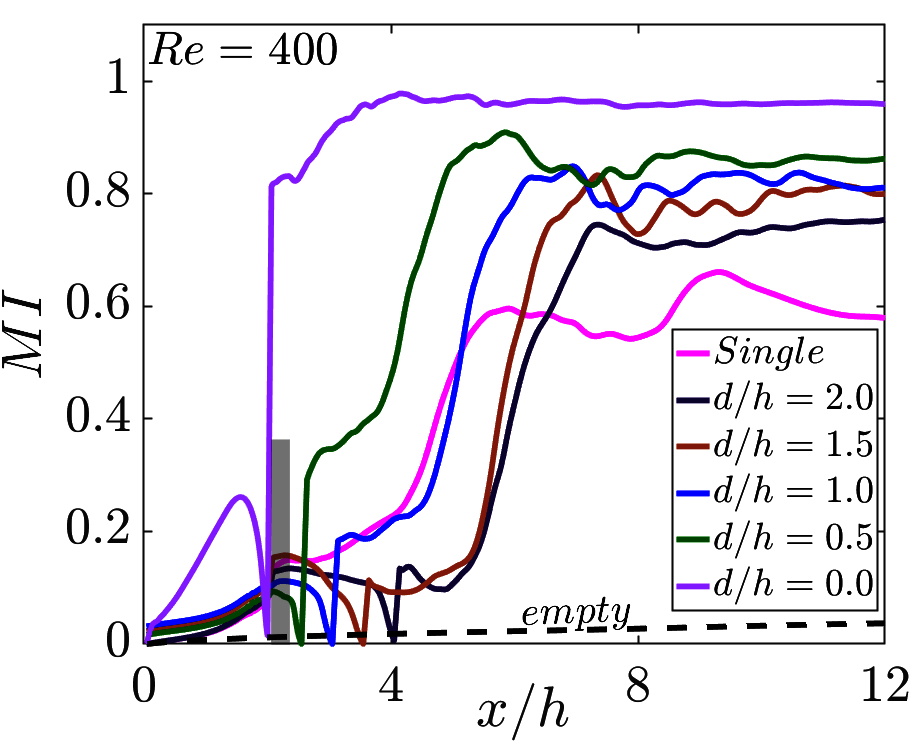
\includegraphics[width=1\linewidth,trim={0cm 0 0 0},clip]{Figures/MI_HL/MI_x_Re400_46.png}
		\begin{overpic}[width=1\linewidth,trim={0cm 0 0 0},clip]{Fig02.pdf}
			\put(0,110){{\parbox{1\linewidth}{$(a)$}}}	
		\end{overpic}
	\end{minipage}
	\begin{minipage}[c]{0.32\linewidth}		
		\begin{overpic}[width=1\linewidth,height=4.5cm]{mesh_def.png}
			\put(3,120){{\parbox{1\linewidth}{$(b)$}}}
		\end{overpic}
	\end{minipage}
	\begin{minipage}[c]{0.31\linewidth}		
		\begin{overpic}[width=1\linewidth,trim={0cm 0 0 0},clip]{GridTest_3c2.png}
			\put(0,118){{\parbox{1\linewidth}{$(c)$}}}
		\end{overpic}
	\end{minipage}
	%	\vspace{0.5cm}
	\caption{(a) Validation of our results with~\cite{Gluck2001}. (b) Streamwise tip deflection at 3 different mesh densities (c) $MI$ and $HL$ attained at the channel length $x=12h$  for cases with $d/h=1.5$ and $Re=800$ for different mesh densities. }
	\label{validation1}
\end{figure*}



\item \textcolor{red}{Figures 8, 10, 11, and 12 are too small. The authors should increase the font size.}

\textbf{Reply}: Thank you for the feedback. We have now increased the figures 8, 10, 11 and 12 for better readability.

\end{enumerate}	


\newpage

\section*{The second referee's comments and actions taken in that regard} 


\textcolor{red}{ This paper presents a study on mixing performance of wall mounted flexible structures in a channel using FSI simulations. The paper is in general well written explaining the flow structures and resulting mixing performance. I have, however, some comments/concerns regarding the presentation of the numerical treatments in this paper:}\\

\textcolor{red}{\textbf{General comments:}}\\


\begin{enumerate}
\item \textcolor{red}{No validation case is presented. The grid independence is very briefly mentioned in the appendix. I expect more discussion to demonstrate the fidelity of the solutions.}

\textbf{Reply}: Apologies for the lack of details on the numerical modelling side. Since these results are an extension of our previous work \cite{Self2019}, we have referred the validation and grid independence details of our simulations to that work. Upon your recommendation, we are adding the following validation results and additional passive scalar based grid validation in the revised manuscript. Thank you.

\subsection*{\textit{Validation and grid independence}} \textit{``To ensure confidence on our numerical solver, we conducted a validation study where we selected a test case involving a plate oscillating in a fluid flow, as illustrated in Figure 12 of~\cite{Gluck2001}. In Figure~\ref{validation1}(a), we present the computed streamwise tip deflection over time and compare it with the results outlined in Section 3.1.2 of~\cite{Gluck2001}. Our simulations showed good agreement with these results. In sequence, we further ensure the accuracy of our results by conducting grid independence results for our study as shown in figure \ref{validation1}(b). We investigated the plates' tip deflection at three different mesh densities and found $\approx1\%$ difference in the values. Based on the convincing results, we proceeded to simulate all the test cases with the present mesh density. We also tested the results in Fig 10 (in the main manuscript) for $d/h=1.5$ and $Re=800$ at different mesh densities to optimize the grid resolution of the scalar field in the domain. We investigated 0.5-1.5 $\times$ the presently used mesh to report Mixing Index and corresponding Head Losses and found the saturation of $MI$ and $HL$ results at the used mesh density."}

\begin{figure*}[h!]
	\begin{minipage}[c]{0.31\linewidth}
		%			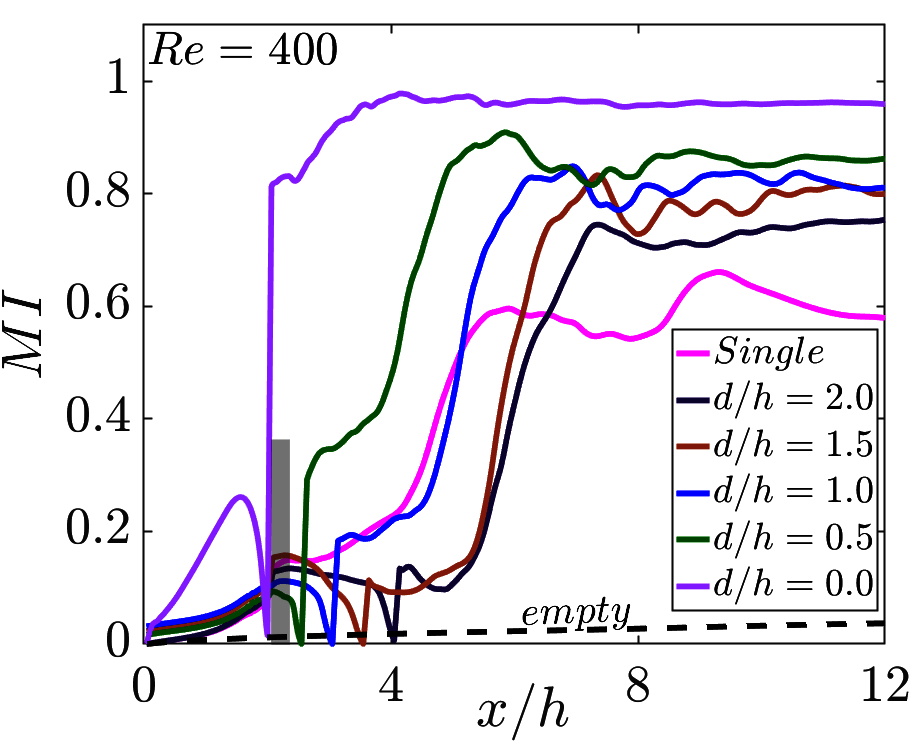
\includegraphics[width=1\linewidth,trim={0cm 0 0 0},clip]{Figures/MI_HL/MI_x_Re400_46.png}
		\begin{overpic}[width=1\linewidth,trim={0cm 0 0 0},clip]{Fig02.pdf}
			\put(-70,110){{\parbox{1\linewidth}{$(a)$}}}	
		\end{overpic}
	\end{minipage}
	\begin{minipage}[c]{0.32\linewidth}		
		\begin{overpic}[width=1\linewidth,height=4.5cm]{mesh_def.png}
			\put(-72,120){{\parbox{1\linewidth}{$(b)$}}}
		\end{overpic}
	\end{minipage}
	\begin{minipage}[c]{0.31\linewidth}		
		\begin{overpic}[width=1\linewidth,trim={0cm 0 0 0},clip]{GridTest_3c2.png}
			\put(-70,118){{\parbox{1\linewidth}{$(c)$}}}
		\end{overpic}
	\end{minipage}
	%	\vspace{0.5cm}
	\caption{(a) Validation of our results with~\cite{Gluck2001}. (b) Streamwise tip deflection at 3 different mesh densities (c) $MI$ and $HL$ attained at the channel length $x=12h$  for cases with $d/h=1.5$ and $Re=800$ for different mesh densities. }
	\label{validation1}
\end{figure*}
	

\item \textcolor{red}{Why have they used a TVD scheme? Are there Gibbs like numerical oscillations near the interface?}

\textbf{Reply}: Thank you for the query. We have Total Variation Diminishing (TVD) schemes for scalars to contain the numerical oscillations at the sharp interfaces because of the moving boundaries to ensure the scalar values to stay realistic and bounded within the range of 0 to 1. TVD schemes effectively handle scalar overshoots and undershoots without introducing excessive numerical diffusion \cite{DEVINCENTIS,Qianyu,CAVALCANTI}.

\item \textcolor{red}{ A fully developed outlet condition is assumed. Justify that.}

\textbf{Reply}: Thank you for pointing out the ambiguity in the manuscript. The query concerns with the phrase: 
``\textit{At the channel outlet, the velocity gradients are set to zero, while the inlet velocity follows a parabolic inflow profile for both the top and bottom half, as previously described.}" 

We need to clarify that the outlet condition is assumed as zero gradient velocity and ambient pressure. The parabolic profiled fully developed velocity condition is given at the bifurcated inlets (left) for each dye. There is no fully developed condition at the channel outlet. Apologies for the ambiguous writing.
We have rephrased the sentence in the revised manuscript for better clarity as: 

``\textit{At the channel outlet, we have assumed zero velocity gradient boundary condition. A parabolic profiled inlet from left is supplied for both the top and bottom half to mimic fully developed flow for the two different concentration fields, as previously described.}"

\item \textcolor{red}{Although the highest considered Re is less than $Re_{cr}$ in channel but is it possible to see onset of transition/turbulence considering the disturbed nature of this flow?}

\textbf{Reply}: Thank you for the insight into underlying physics of the setup. With flexible moving parts and increased shear effects it is expected to discover zones of transitions in the flow domain. In fact, the whole motivation of this problem emerges from this idea of onset of turbulence. This investigation is the continuation of our previous study \cite{Self2019}, where we have shown profound details on the flow transition by investigating the energy cascading effect in terms of energy dissipation rates and discovered the intermittent turbulence in the flow because of both the core and boundary layer zones. The ‘stir’ created in the flow by different scales of
motion helps in redistributing the scalar fields. Eventually,
all the gradients smear at the small scales due to the molecular diffusion; thus, thorough mixing takes place. The flow instabilities help in amplifying the local flow fluctuations and
leads to an increased mixing rate. 
In compliance with the results shown in our previous work, we find that the case with $d/h=0.0$ shows highest $MI$ for all $Re$ cases as it showed highest energy dissipation rates (see Fig. 17 in \cite{Self2019}).


We have added a short description regarding this in our main manuscript in page 6:

 \textit{``This result builds on our previous study \cite{Self2019}, where we detailed how energy cascades in the flow, measured through energy dissipation rates, and identified intermittent turbulence caused by both the core flow and boundary layers. The stirring effect created by motions at different scales redistributes scalar fields, while molecular diffusion eventually smooths out the gradients at small scales, resulting in thorough mixing. Flow instabilities amplify local fluctuations, increasing the mixing rate. Consistent with our earlier findings, the case with $d/h=0.0$ shows the highest mixing index (MI), as it also exhibited the highest energy dissipation rates (see Fig. 17 in \cite{Self2019}).}"


\end{enumerate}



				\begin{thebibliography}{100} % 100 is a random guess of the total number of
	%references
	\bibitem{Self2019} Gaurav Singh and Rajaram Lakkaraju, ``Wall-mounted flexible plates in a two-dimensional channel trigger early flow instabilities", \emph{Phys. Rev. E}, American Physical Society, Vol. 100, 2 pp. 023109, Aug 2019.
	\bibitem{CAVALCANTI} José Rafael Cavalcanti and Michael Dumbser and David da Motta-Marques and Carlos Ruberto {Fragoso Junior}, ``A conservative finite volume scheme with time-accurate local time stepping for scalar transport on unstructured grids", \emph{Advances in Water Resources}, Vol. 86, 2 pp. 217-230, 2015.
	
		\bibitem{Qianyu} Qianyu Zhang, ``Implementation and Validation of TVD Schemes for Modelling of Multiphase Flow", \emph{Dissertation, University of Albert}, 2019.
		
			\bibitem{DEVINCENTIS} Brian DeVincentis and John Thomas, ``A conservative finite volume scheme with time-accurate local time stepping for scalar transport on unstructured grids", \emph{Computers \& Mathematics with Applications}, Vol. 144, pp. 1-11, 2023.
	
		
		\bibitem{Gluck2001} Markus Gl{\"{u}}ck, Michael Breuer, F. Durst, A. Halfmann and Ernst Rank, ``Computation of fluid–structure interaction on lightweight structures" \emph{Journal of Wind Engineering and Industrial Aerodynamics}, Vol. 89, 14-15 pp. 1351-1368, 2001.  
		
		\bibitem{Antognoli} Matteo Antognoli and Sara {Tomasi Masoni} and Alessandro Mariotti and Roberto Mauri and Elisabetta Brunazzi and Chiara Galletti, ``Investigation on steady regimes in a X-shaped micromixer fed with water and ethanol" \emph{Chemical Engineering Science}, Vol. 248, 0009-2509 pp. 1117254, 2022. 
				
		\bibitem{Orsi} Gianni Orsi and Mina Roudgar and Elisabetta Brunazzi and Chiara Galletti and Roberto Mauri, ``Water–ethanol mixing in T-shaped microdevices" \emph{Chemical Engineering Science}, Vol. 248, 0009-2509 pp. 174-183, 20213. 
		
		\bibitem{Galletti} Matteo Antognoli and Sara {Tomasi Masoni} and  and Roberto Mauri and Elisabetta Brunazzi and Chiara Galletti, Alessandro Mariotti,Lorenzo Siconolfi, Roberto Mauri and Elisabetta Brunazzi, ``Investigation on steady regimes in a X-shaped micromixer fed with water and ethanol" \emph{Chemical Engineering Science}, Vol. 97, 2 pp. 528-541, 2019. 
 

\end{thebibliography}
	

    
\end{document}